%!TEX root = ../thesis.tex
\chapter{Experiments}
\label{chap:experiments}
In this chapter, both proposed heterogeneous pc-stable algorithm approaches are evaluated. Therefore, we conduct a series of experiments, which show how effective the approaches execution times are and where possible problems occur with the proposed solutions. Furthermore, two different systems are used for the evaluation to elaborate the hardware dependency of the heterogeneous version. First, we describe the detailed setup of the following experiments in Chapter \ref{chap:setup}. Then in Chapter \ref{chap:est_speedup} an estimation on the potential speedup of the proposed solution is done. In the end, benchmarks with their results are explained in Chapter \ref{chap:benchmarks}.

\section{Setup}
\label{chap:setup}
All experiments are based on the same dataset, which is also used in the experiments of Perscheid et al. \cite{perscheidIntegrativeGeneSelection2018}. The dataset is taken from The Cancer Genome Atlas (TCGA) \cite{weinsteinCancerGenomeAtlas2013}. Genes with more than 30\% missing values are filtered out. The remaining data is normalized and log-transformed. The original dataset consists of 55 573 variables. While the runtime of the PC stable algorithm grows exponentially with the variable count, subsets of the dataset are used for evaluation. The subset sizes chosen for the evaluation are 1000 variables, 10 000 variables, and 45 000 variables. The 1000 variables dataset is used to represent small datasets and will be called TCGA-1000. The 10 000 variables dataset is a large dataset that does not fill the memory of the system's GPU and will be called TCGA-10000. The 45 000 variables dataset is used to show the effects of GPU memory overflow on the algorithms execution time in this evaluation and is called TCGA-45000.

Terminology has to be defined to introduce the systems used for the experiments. A NUMA node is defined as some CPU and each non CPU device directly connected to that CPU so that there is no indirection in memory access from that CPU. NUMA nodes are essential for interconnection speed because multiple interconnects between devices in a system can be avoided. NUMA nodes can be pinned for execution so that the executed program can only use the resources of that NUMA node. Pinning the execution of a program to a single NUMA node while the system incorporates multiple CPUs leads to fewer cores available for execution because the other CPUs' resources cannot be used.

The type of interconnection between processing units defines the speed with which processors can communicate. One important metric for interconnect speed is the bandwidth or throughput. While PCIe 3.0, which is used as a GPU-CPU in the following system (Figure \ref{fig:delos_arch}), has a maximum bandwidth of 15,75 GB/s, NVLink 2.0 is faster with a maximum of 25 GB/s \cite{zargesEvaluationOnNodeGPU}. The bandwidth gap between PCIe and NVLink grows even larger when multiple NVLink lanes are combined and used together as a single interconnect. Such NVLink combinations are often used in modern high-performance systems generating a maximum bandwidth of 50 GB/s or higher. NVLink is an interconnect standard designed for GPU-GPU connections but is also used as CPU-GPU interconnects in dedicated Power systems by IBM \cite{liEvaluatingModernGPU2020}. Interconnects between CPUs like UPI or X-Bus 4B are generally avoided because there is almost always a faster and more direct way to access data in memory when data management of the algorithm is done right. For complete avoidance and impact measuring of an additional CPU-CPU interconnect, experiments are done using a single pinned NUMA node.

\begin{figure}[H]
  \caption{System 1 Structure - Delos}
  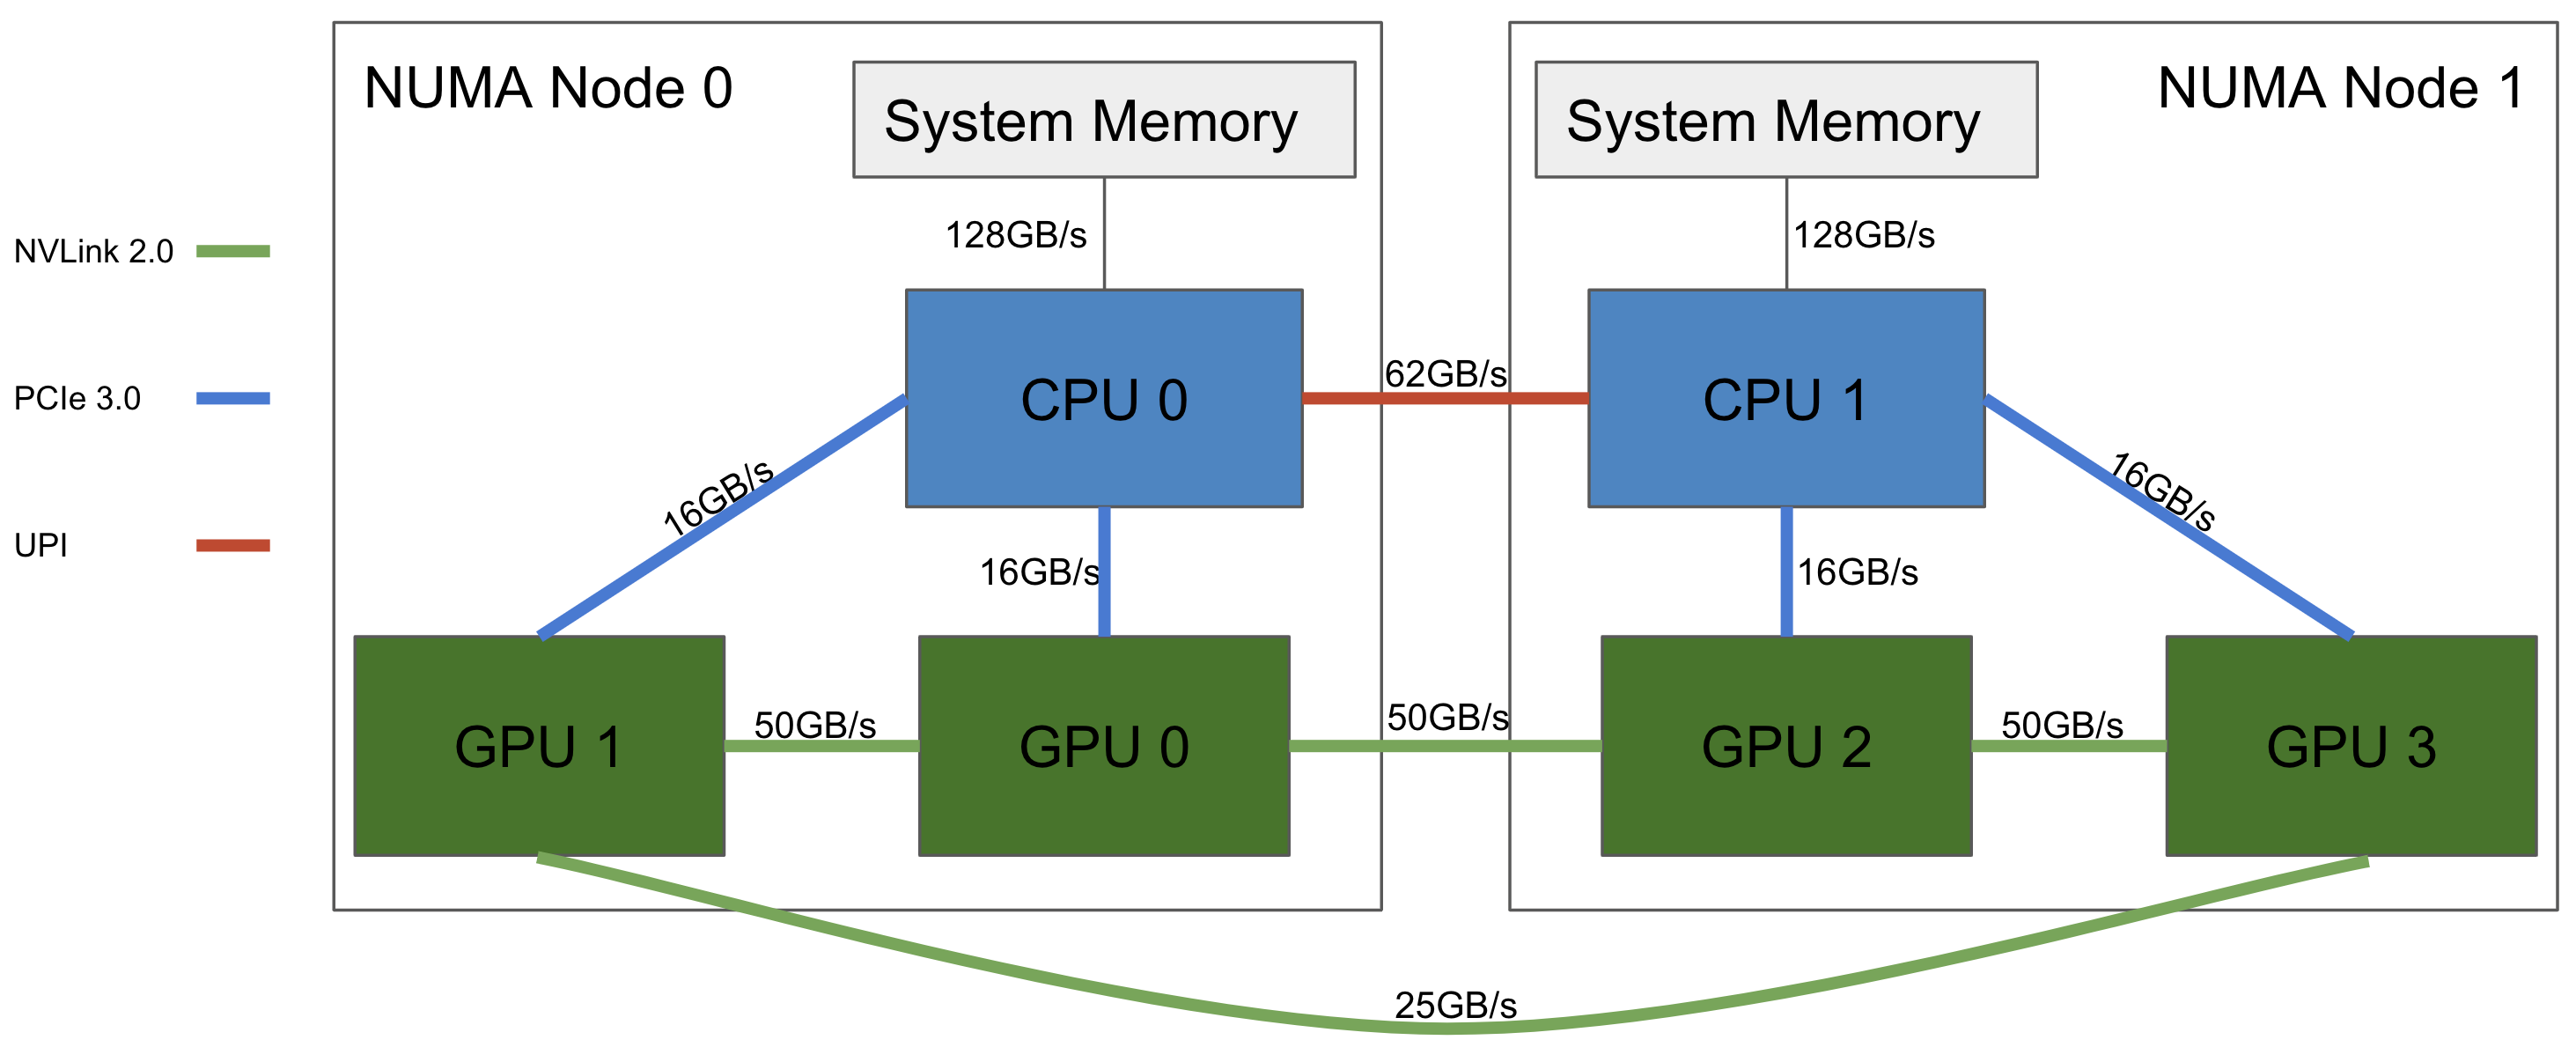
\includegraphics[width=\textwidth]{figures/delos_system_arch.png}
  \centering
  \label{fig:delos_arch}
\end{figure}

Two different systems are used for the evaluation. One system depicted in Figure \ref{fig:delos_arch}, which will be called Delos in the following, consists of 4 Nvidia Tesla V100 GPUs with each 32GB of HBM2 memory and 2 Intel Xeon Gold 6148 CPUs with each 755GB of DDR4 memory. The Tesla V100 GPU clock rate is 1,53 GHz. It contains 80 Streaming Multiprocessors which each can execute a maximum of 2048 threads concurrently \cite{NVIDIATESLAV1002017}. The Intel Xeon Gold 6148 has 20 cores with a clock rate maximum of 3,70 GHz. Each core has two so-called hyper threads so that the CPU can execute 40 threads concurrently. Because of the association between NUMA nodes and CPUs, pinning to a single NUMA node also reduces the accessible hyper threads to 40. The CPU-GPU interconnect is PCIe 3.0 and the GPU-GPU interconnect is doubled NVLink with 50 GB/s bandwidth \ref{fig:delos_arch}.


\begin{figure}[H]
  \caption{System 2 Structure - AC922 \cite{ganesannarayanasamyPowerAIDeepDive12:39:24UTC}}
  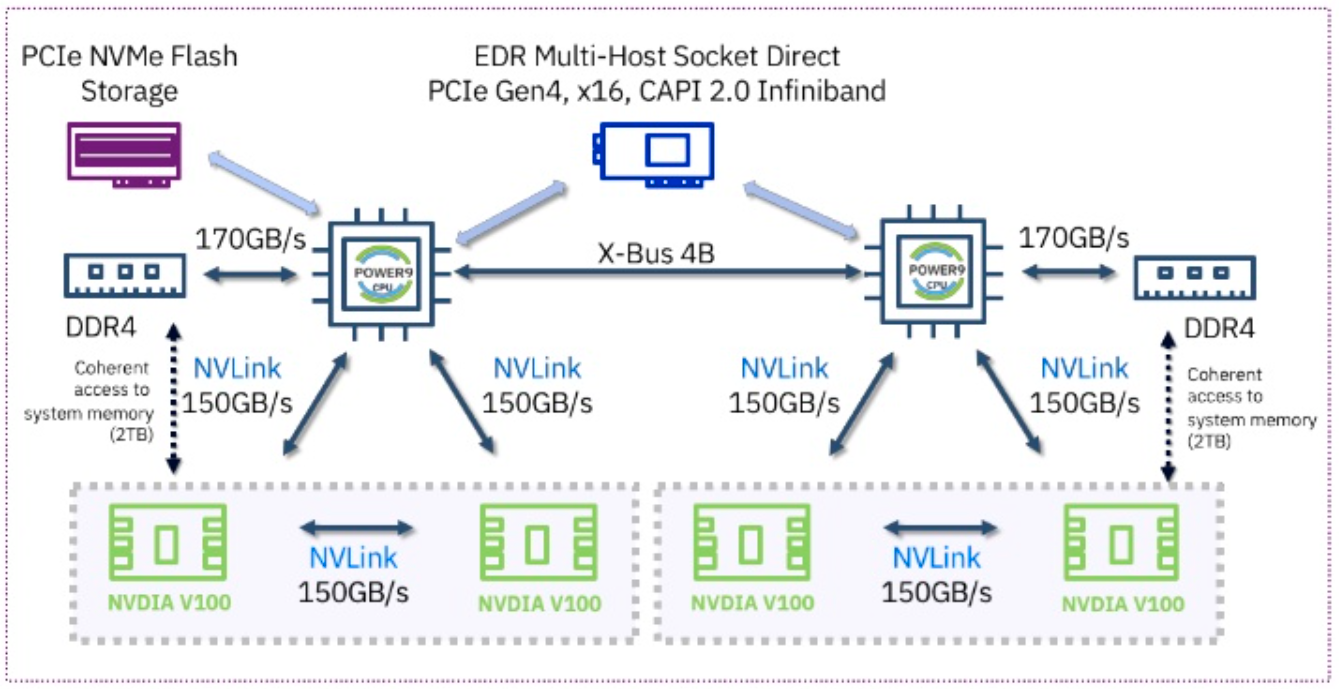
\includegraphics[width=\textwidth]{figures/ac922_system_arch.png}
  \centering
  \label{fig:ac922_arch}
\end{figure}

The second system depicted in Figure \ref{fig:ac922_arch}, which will be called AC922 in the following, is a high-performance computing system developed in collaboration with IBM and Nvidia \cite{caldeiraIBMPowerSystem}. It incorporates the same GPUs as the Delos system (4xNvidia Tesla V100) and two IBM Power9 processors. Each Power9 processor has 16 cores with a clock rate maximum of 4 GHz, which, by using SMT4 multithreading, can execute 64 threads concurrently. 256GB DDR4 RAM is connected to each CPU.

Through the collaboration of IBM and Nvidia, the interconnect between a CPU and GPU in this system is NVLink \cite{NVLink2021, zargesEvaluationOnNodeGPU} with a bandwidth of 150GB/s in contrast to the Delos PCIe 3.0 16GB/s interconnect. NVLink 2.0 is also twice as fast latency-wise compared to PCIe 3.0 \cite{liEvaluatingModernGPU2020}. Both systems' latency and throughput differences allow evaluating bottlenecks regarding interconnect speed in this heterogeneous computation scenario.
Furthermore, the collaboration brings other features which a heterogeneous computing application can benefit from, such as Adress Translation Services \cite{ibmpower9nputeamFunctionalityPerformanceNVLink2018} unifying the GPU and CPU page table, native atomics support for system-wide accessible memory, and direct GPU memory access by the CPU \cite{UNIFIEDMEMORYP9}.

The following experiments only use one GPU for execution, even if the proposed algorithm can be executed on multiple GPUs at once. Therefore parameters, such as GPU-GPU memory handling and interconnect technology, do not influence the CPU-GPU computation results. Some benchmarks are pinned to the NUMA node closest to the executing GPU to limit interconnect effects unrelated to the direct CPU-GPU connection. Both systems' CPUs are directly connected to two GPUs, using only half the cores and memory while pinned to one NUMA node. The largest dataset used with the size of 36GB$\sim$ will not be the limiting factor for the CPU's associated memory of 755GB on Delos and 256GB on AC922. On the other hand, 36GB$\sim$ of data will fill the GPU's memory of 32GB which is intentional behavior as said above.

The following table shows the tools and libraries used for the experiments:
\begin{table}[h!]
  \centering
  \begin{tabular}{||c | c||} 
   \hline
   Delos & AC922 \\ [0.5ex] 
   \hline\hline
   GCC 8.4.0 & GCC 8.3.1 \\
   CUDA 11.3 & CUDA 11.3 \\ 
   CMake 3.20.2 & CMake 3.20.2 \\
   Armadillo 10.5.1 & Armadillo 10.5.1 \\
   Boost 1.65.1 & Boost 1.76.0 \\ [1ex]
   \hline
  \end{tabular}
  \caption{Tools and libraries and their versions used in the experiments}
  \label{table:libversions}
\end{table}

CMake is used as a build tool simplifying the build process, which can handle CUDA code compilation and optimization for specific Nvidia GPUs used. GCC is used as the host compiler for the C++ code, with the versions already existing on the system. The CUDA compiler and libraries are provided by the CUDA Toolkit version 11.3. The CPU side mathematical calculations such as the pseudoinverse are done using Armadillo C++, an abstraction of BLAS libraries, so that best performance is achieved on each system. Boost is used for creating the command line interface of the application and for numerical helper functions.

Further, the following flags were passed to GCC on the systems:
\begin{itemize}
  \item Delos: -O3 -DNDEBUG -march=native -mtune=native
  \item AC922: -O3 -DNDEBUG -flto -fpeel-loops -funroll-loops -ftree-vectorize -ffast-math -mcpu=power9 -mtune=power9
\end{itemize}
The flags used on the AC922 system are recommended by IBM for optimized binaries \cite{LinuxIBMPower}. NVCC, the Nvidia CUDA compiler, gets passed the same flags on both systems (-O3 -DNDEBUG -lineinfo). Additionally, CMake automatically sets the correct flags to compile for best optimization on the V100 architecture.

Runtime measurements are done with the chrono standard library of C++ by saving the starting points system time and subtracting the starting points time when the measurement is finished. The accuracy of those measurements is rounded to milliseconds. The measurement code is used on multiple abstractions, measuring the load-balancing, GPU and CPU execution times, the whole level, and the entire PC algorithms execution time.
Each experiment based on the TCGA-1000 dataset is done in five iterations.  Because of the statistical influence of outliers on the mean, outliers in the execution times, extracted in the context of the dataset size, are rerun and measured again. The mean of all iterations execution times for each measured part is taken. Those calculated means are then used for the following visualizations.

\section{Estimating the Speedup}
\label{chap:est_speedup}
Analyzing the TCGA-1000 dataset while executing could lead to a potential estimation of the theoretical speedup possible through the heterogeneous execution. In Chapter \ref{chap:agglo} where the Agglomeration stage of Foster's Methodology is applied to the PC-stable algorithm, the execution time of an edge is estimated by the length of the containing adjacency list.

\begin{figure}[H]
  \caption{Boxplot of the adjancency row lengths at the start of each level based on the TCGA-1000.}
  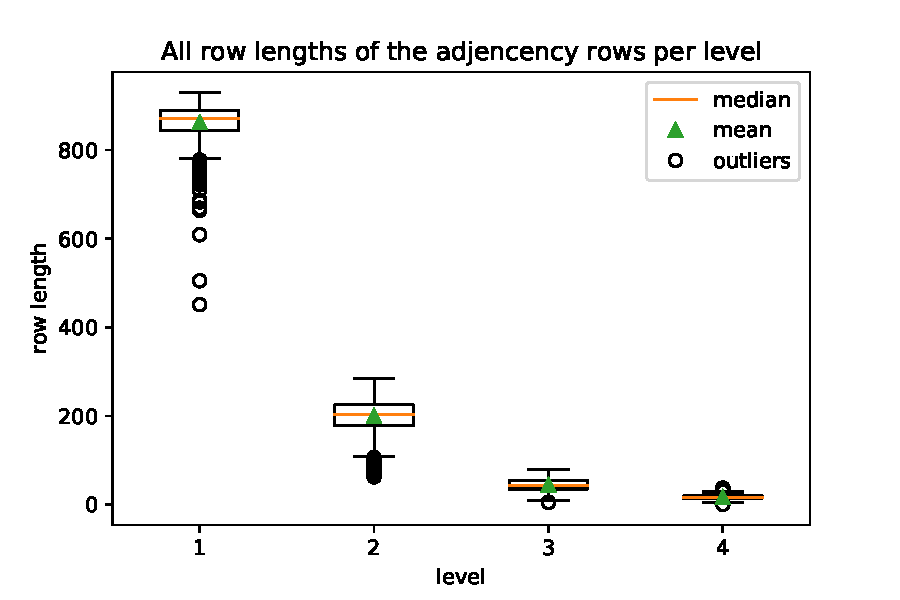
\includegraphics[width=\textwidth]{figures/rowlength_bxplt.pdf}
  \centering
  \label{fig:rowlength_bxplt}
\end{figure}

When plotting the length of each vertexes adjacency list before the level is executed in Figure \ref{fig:rowlength_bxplt}, a decline in edge deletions can be seen. The higher the level, the fewer edges are deleted. Most deletions happen in level one. Through rising test cases in higher levels with growing separation set combinations, the row length is not suitable anymore for estimating the execution time of a warp on the GPU. As said in the Agglomeration Chapter, the maximum iterations can be calculated using the maximum CI-tests that could be done for that row with a given level. The maximum CI-tests directly estimate the maximum execution time for each edge in that row and indicate the possible speedup through the heterogeneous PC algorithm variant.

\begin{figure}[H]
  \caption{Boxplot of the maximum iterations needed for an edge in that row by a GPU warp. Calculated using the row lengths of Figure \ref{fig:rowlength_bxplt}.}
  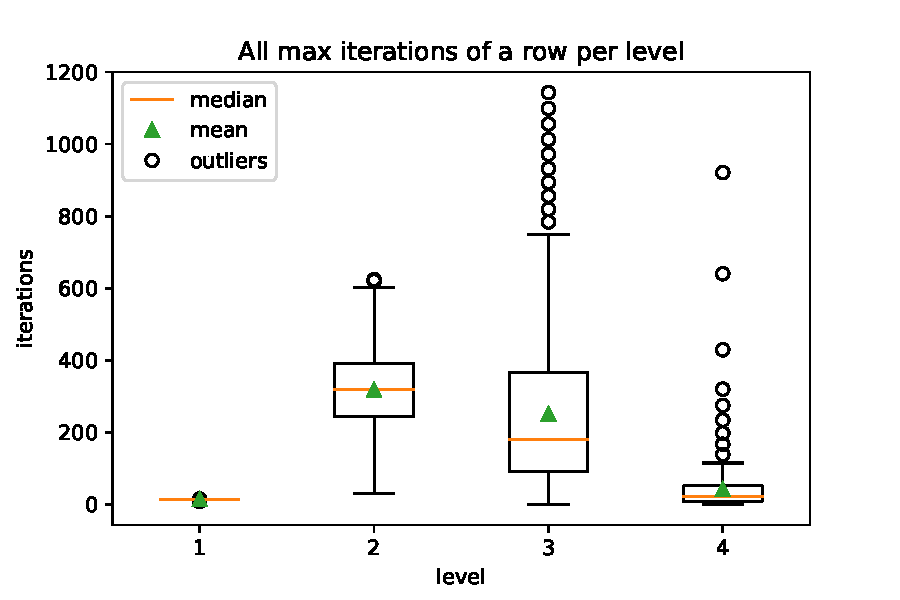
\includegraphics[width=\textwidth]{figures/iterations_bxplt.pdf}
  \centering
  \label{fig:iterations_bxplt}
\end{figure}

In Figure \ref{fig:iterations_bxplt} the calculated maximum iterations needed by a GPU warp can be seen. The iterations data is based on the row lengths of Figure \ref{fig:rowlength_bxplt}. Looking at the otuliers, which should significantly impact the execution time by being the sequential parts of the parallelized levels, placing those on the CPU should speed up the GPU's execution time. Levels one and two do not show strong outliers and therefore might not be more performant executed heterogeneously. Levels three and four, in contrast to the earlier levels, do have strong outliers. In level three, a theoretical speedup of around 30\% could be achievable by cutting those outliers and placing them on the CPU. In level four, around 80\% of the execution time could be cut using the heterogeneous PC algorithm variant.

\section{Benchmarks}
\label{chap:benchmarks}
For each system, basic experiments for both approaches without system side modifications are done first to determine the relevance and effectiveness of those approaches. To analyze hardware-specific effects on the experiments, more detailed benchmarks are done later, such as tests with a modified thread count used for the CPU execution.
The first approach, which is called pre-balanced, will be tested and compared to the GPU-only execution of the algorithm. Additionally, migrating edges after each level could prevent page migrations between the CPU and GPU, and pinning the execution to some NUMA node is also  tested.

The same tests are then done for the workstealing approach, where a test for atomic usage is added. Atomics are used in the workstealing approach to mark and determine if an execution unit already started a task to prevent processing tasks twice. This test case is added to compare the overhead of using atomics in comparison to processing tasks twice.

Those described experiments are done on both the Delos system and the AC922 system. Each test relying on the TCGA-1000 dataset is executed five times, and for the final result, the mean of all results is calculated as described in the setup. On the Delos system, further experiments to evaluate the scalability of the approaches are done using large datasets, which are iterated only once because of their long execution times.

\subsection{Benchmarks Delos}
The following benchmarks on Delos using both approaches are plotted and explained.

\paragraph{Pre-Balanced TCGA-1000 Benchmarks}
\begin{table}[H]
  \centering
  \begin{tabular}{||c | c | c | c||} 
   \hline
    & Execution time (ms) & $\Delta$ & $\Delta$ speedup in \% \\ [0.5ex] 
   \hline\hline
   GPU-only & 16290.8 & 0 & - \\
   Pre-Balanced & 15853.8 & -437 & 2,68 \\ 
   No post level migrations & 15821.8 & -469 & 2,96 \\
   NUMA node pinned & 16839.6 & 548,8 & -3,36 \\ [1ex] 
   \hline
  \end{tabular}
  \caption{Pre-Balanced execution time results (Delos)}
  \label{table:preb_delos}
\end{table}
The first experiments using the pre-balanced approach seen in \ref{table:preb_delos} show that there is a slight performance boost of 2,9\% without pinning the NUMA node compared to the GPU-only variant possible. While pinning the NUMA node, there is even a slow down seen, which tells us that the processing power of the lost cores has slowed the execution, and more cores should help speed up the execution. 

The effect of deleting edges during or after the level on the execution time is negligible. So the interconnect bottleneck does not hit the performance in a meaningful way when edges of different rows are processed by GPU and CPU, supported by the little to no effect of migrating edges after level execution. 

Additionally, the count of rows placed on the CPU by the load-balancer had to be tuned carefully for the best performance. The row count of rows balanced on the CPU is 14 rows in levels one and two and 8 rows in levels three and four, which is small compared to the maximum of 1000 rows.

This volatility makes tuning the pre-balanced approach hard, especially for large datasets where the PC stable algorithm can execute for hours or days. Multiple tuning executions might not be feasible in such situations because this threshold might change a lot for different datasets, which could lead to more sparse rows.

\paragraph{Workstealing TCGA-1000 Benchmarks}
\begin{table}[H]
  \centering
  \begin{tabular}{||c | c||} 
   \hline
    & Execution time (ms) \\ [0.5ex] 
   \hline\hline
   GPU-only & 16290.8 \\
   Workstealing & 15796.8 \\ 
   Workstealing without postponed edge migrations & 15892.2 \\
   Workstealing without atomics & 23551.0 \\
   Workstealing NUMA pinned & 16266.4 \\ [1ex] 
   \hline
  \end{tabular}
  \caption{Workstealing execution time results (Delos)}
  \label{table:workst_delos}
\end{table}
Experiments with the workstealing approach seen in \ref{table:workst_delos} show a 3,1\% performance boost in comparison to the GPU-only execution, which is similar to the pre-balanced approaches result, even if there should be dynamic scheduling overhead. Postponing the migration of the edge deletion does not impact the execution time, whereas the benchmark without atomics shows a slowdown of $\sim$33\ in comparison to using atomics. The slowdown of the execution while not using atomics presumably happens because tasks are processed multiple times. Changes to the flags annotating tasks that are being processed must be migrated via pages between the processors.

\paragraph{Comparing the Workstealing and Pre-Balanced Benchmarks}
Comparing the pre-balanced approaches and the workstealing approaches results, both seem similarly effective for speeding up the PC-stable variant. Still, workstealing and dynamic scheduling are more flexible because they do not need to be tuned for the dataset being used, and a speedup is still seen. Due to the flexibility, further tests on the Delos system are done using the workstealing approach.

\paragraph{Threaded CPU Execution Scaling with TCGA-1000}
\begin{figure}[H]
  \caption{Testing the CPU side parallelizability of the workstealing approach on Delos. Points of interests marked with vertical colored lines.}
  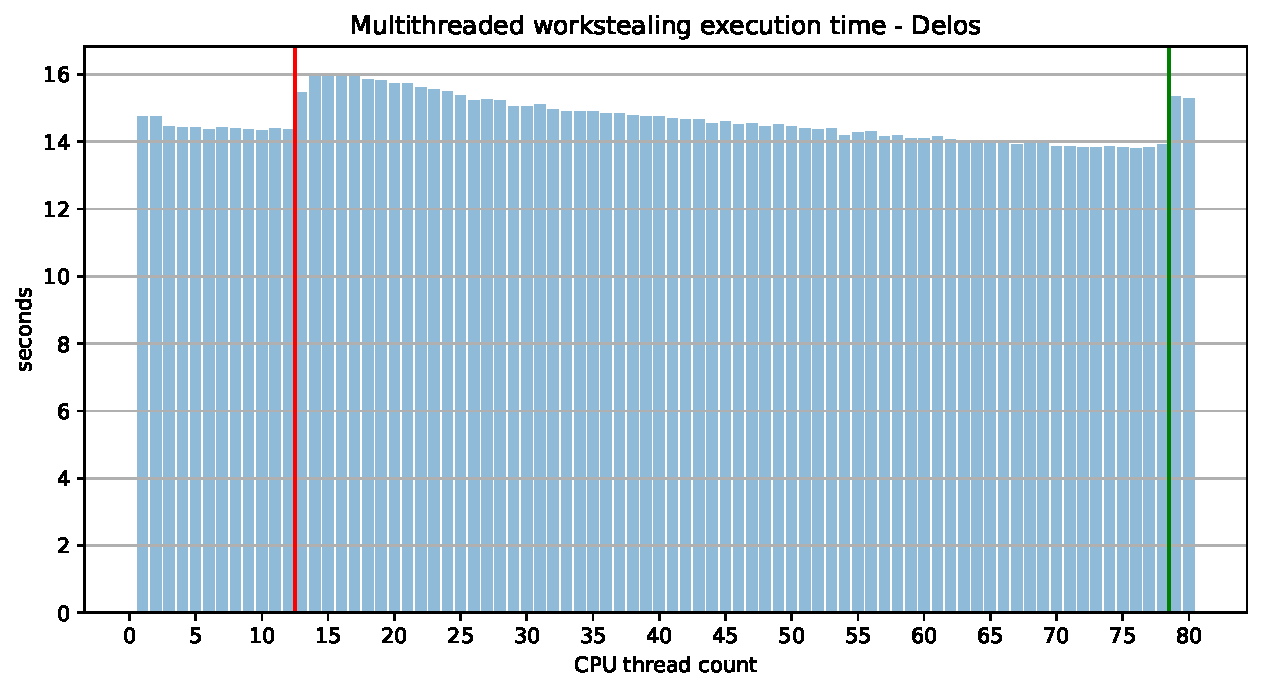
\includegraphics[width=\textwidth]{figures/threaded_wsteal.pdf}
  \centering
  \label{fig:wstealing_threaded_delos}
\end{figure}

The implementation of the CPU execution is parallelized with OpenMP, a library that allows easy tuning of the thread count that is spawned for execution. In the following experiment, the parallelizability of the CPU execution can be seen in Figure \ref{fig:wstealing_threaded_delos}.
The peak at 79/80 threads, marked with a green vertical line, is expected because there is also the main thread running used for orchestration, and additionally one thread per GPU is used for GPU synchronization. With 80 plus at least additional 2 threads running, there are not enough execution units available to run all threads without collisions. Therefore the maximum number of threads that the CPU tasks execution should use is 78 (using one GPU), so that the sum of threads used is 80 running on the 80 hyperthreads of Delos.

While a performance boost can be seen for additional threads spawned, there is another peak of execution time at around 12 threads, marked with a red vertical line. We could not find a proper reason for that behavior but speculate that it is caused by bad optimization, which could be an interconnect bottleneck hit with the two NUMA nodes involved or the system-wide synchronization through atomics. 78 thread execution is the fastest, but not by far, and therefore might not be suitable compared to one thread in energy-efficient environments because using more cores of a CPU means effectively using more watt \cite{saravananStudyFactorsInfluencing2011}. Using 78 threads is around 5\% faster than using a single thread.

Looking at the workstealing performance, the speedup of 78 threads workstealing compared to GPU-only is $\sim$16,6\%.

\paragraph{Workstealing TCGA-10000 and TCGA-45000 Benchmarks}
\begin{table}[H]
  \centering
  \begin{tabular}{||c | c | c||} 
   \hline
   Variable count & 1 thread speedup factor & 78 threads speedup factor \\ [0.5ex] 
   \hline\hline\hline
   1000 & 1,11x & 1,17x \\
   10 000 & 0,95x & 0,96x \\ 
   45 000 (only level 0 and 1) & 1,06x & 6,61x \\ [1ex] 
   \hline
  \end{tabular}
  \caption{Workstealing execution time results (Delos)}
  \label{table:workst_delos_scaling}
\end{table}

Looking at the scalability of the workstealing approach by running benchmarks on larger datasets, it can be seen that the approach might not scale well. At 10 000 variables, there is even a slowdown. This slowdown can be explained by the rising data migration between the CPU and the GPU with more variables to be randomly accessed, and the limited CPU-GPU interconnect throughput. More variables also produce more row length peaks, which are less likely to be an outlier because of the higher possibility of occurring peaks.
The GPU-only execution is presumably faster due to the better memory access times without having to migrate data.

While the dataset based on 10 000 variables does not exhaust the memory associated with the GPU, the 45 000 variable dataset does. By exhausting the GPU memory, the CUDA runtime has to swap memory in and out while accessing because there is always a part of the dataset, which cannot be held in memory. This swapping process is usually slow because the CPU-GPU interconnect is used and does get triggered if there is some random access pattern \cite{gangulyAdaptivePageMigration2020, kimBatchAwareUnifiedMemory}.

The CPU still holds the whole data in system memory and can access the data fast. The heterogeneous computing approach is 6,61 times faster than the GPU-only variant because the memory overflown GPU is slower in this case. The CPU can help more by having faster access times on the data without the data migration happening.
Since the raw computing power is the most critical part of the CPU in this scenario, using more threads speeds the computation up.

\paragraph{Level-Wise Workstealing Benchmarks}
\begin{figure}[H]
  \caption{Comparing the level-wise speedup factor of the pre-balanced and workstealing approach to GPU-only execution}
  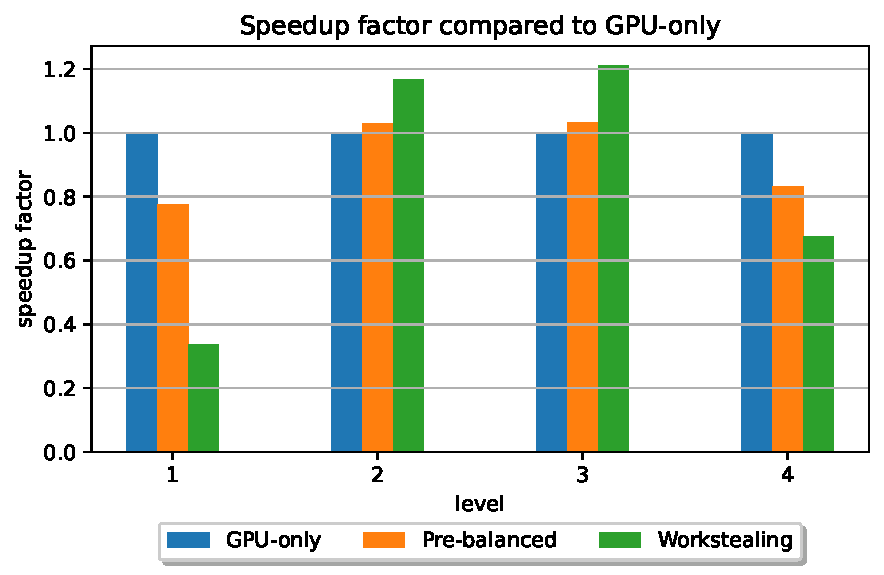
\includegraphics[width=\textwidth]{figures/levelwise.pdf}
  \centering
  \label{fig:levelwise_delos}
\end{figure}

By comparing the speedup level-wise in Figure \ref{fig:levelwise_delos} it is clear that the heterogeneous computing speedup impacts levels 2 and 3 through the CPU. Levels 1 and 4 are slower than GPU-only when executed heterogeneously because there are less to no execution-time outlier tasks in the data that can be placed on the CPU. In levels 2 and 3, there are more significant and more performance impacting outlier tasks. The influence of levels 1 and 4 is negligible due to the small share of 1\% in the execution time. Nevertheless, the best performance is achievable through executing only levels 2 and 3 via heterogeneous computing. The level-wise effect is even more substantial for the workstealing approach in comparison to the pre-balanced approach.

Interestingly the most tasks are stolen in level 1 by the CPU. While the CPU steals around 90 000 tasks in level 1, where the additional help of the CPU slows the execution, the CPU steals around 4000 tasks in level 2 and 1000 in level 3. The difference of stolen tasks between levels 1 and 2/3 is expected because tasks in higher levels are slower on average, and the CPU takes the longest tasks on purpose. This difference in processed tasks on the CPU supports the argumentation of the most effective outliers of levels 3 and 4 (cf. Chapter \ref{chap:est_speedup}), because more outliers, which generally take longer, are done on the CPU in those levels.

\begin{figure}[H]
  \caption{Comparing the level-wise speedup factor of the workstealing approach to GPU-only execution with the 10 000 variables TCGA dataset}
  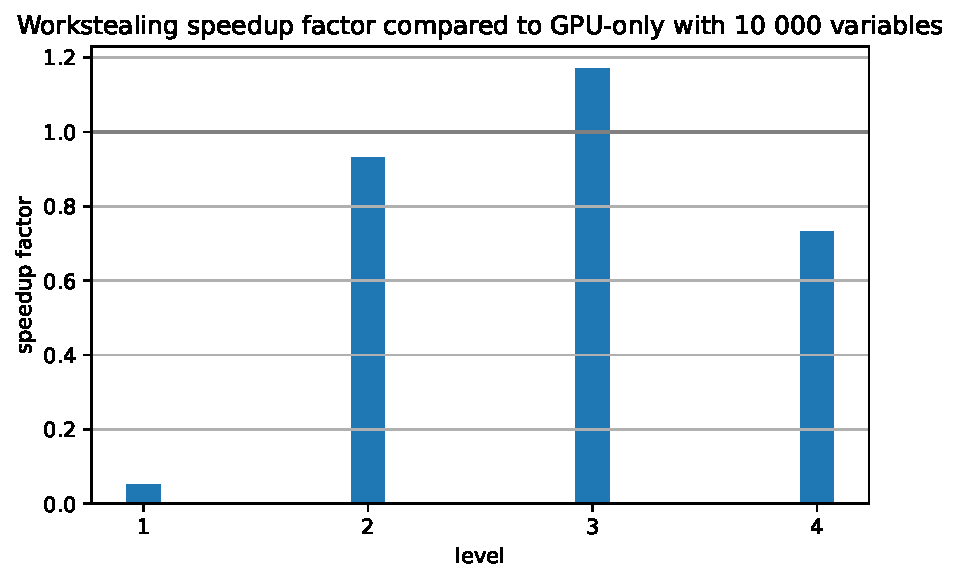
\includegraphics[width=\textwidth]{figures/levelwise_scaled.pdf}
  \centering
  \label{fig:levelwise_scaled_delos}
\end{figure}


The scaling issue seen in the TCGA-10000 dataset benchmark \ref{table:workst_delos_scaling} can be analyzed further by also inspecting the level-wise performance \ref{fig:levelwise_scaled_delos}. In the benchmarks speedup factor result, a performance improvement of around 17,1\% can be obtained in level 3 using the workstealing approach.

\subsection{Benchmarks AC922}
After exploring both approaches on the Delos system, a different look at the CPU-GPU interconnect bottleneck is evaluated by doing comparable benchmarks on the AC922, whose interconnect is faster by relying on NVLINK in contrast to Delos, which relies on PCIe. Native system-wide atomics should also show in the workstealing benchmarks.
While the GPU built into both systems is the same Nvidia V100 GPU, the built-in CPUs are different and might impact the benchmarks.

While the Intel Xeon CPU included in the Delos system is x86\_64 architecture based, the Power9 CPU, which is included in the AC922 system, is based on the ppc64le architecture. Through the different architectures of both CPUs, different optimizations are done, which can influence execution times. Those optimizations include different SIMD instruction set extensions (e.g., AVX versus AltiVec), different instruction set designs (CISC versus RISC), or different core-based task-level parallelism technologies (hyperthreading versus SMT Mode) \cite{AnalysisX86Vs}.

\paragraph{TCGA-1000 Benchmarks for both approaches}
\begin{table}[H]
  \centering
  \begin{tabular}{||c | c||} 
   \hline
    & Execution time (ms) \\ [0.5ex] 
   \hline\hline
   GPU-only & 16577.2 \\
   Pre-Balanced & 2681473.8 \\ 
   Pre-Balanced NUMA pinned & 919603.2 \\
   Workstealing & 415608.2 \\
   Workstealing NUMA pinned & 148823.8 \\ [1ex] 
   \hline
  \end{tabular}
  \caption{Pre-balanced and workstealing execution time results (AC922), Max OMPThreads, Pre-Balanced tunign same as in Delos benchmarks}
  \label{table:bench_ac922}
\end{table}

Benchmarks with both approaches, as shown in Table \ref{table:bench_ac922} indicate that there is a new bottleneck occurring on the AC922 system. The AC922 system benchmarks for both approaches show a significant slowdown. Compared to the workstealing approaches results, the pre-balanced approach is slower with a more significant gap than the GPU-only execution. This gap may indicate that the CPU of the system may be at fault for a large portion of the slowdown, which is supported by the fact, that NUMA pinning, which halves the core count, speeds up the performance of both approaches a lot.

The pre-balanced approach places rows on each execution unit/core of the processor. The parameter that controls this behavior is tuned the same way for this benchmark as in the Delos systems benchmarks for comparison purposes.
% In the pre-balanced approach, the GPU should finish at least simultaneously as the GPU-only variants GPU should since there is no difference in execution. Therefore the slowdown can only occur through a longer load-balance duration of the CPU execution, taking way longer than the GPU execution.

% Looking at the measurements of the pre-balanced execution, the load-balance duration is negligible because the time measurement mechanism does round the time to 0 milliseconds for each TCGA 1000 variables execution. In both the pre-balanced and the workstealing approaches measurements, a disparity between the CPU and the GPU execution time can be seen.

\paragraph{SMT, Threading and NUMA Benchmarks}
\begin{figure}[H]
  \caption{Comparing the workstealing approach pinned to a NUMA node, with different thread counts for OpenMP and different SMT settings (AC922)}
  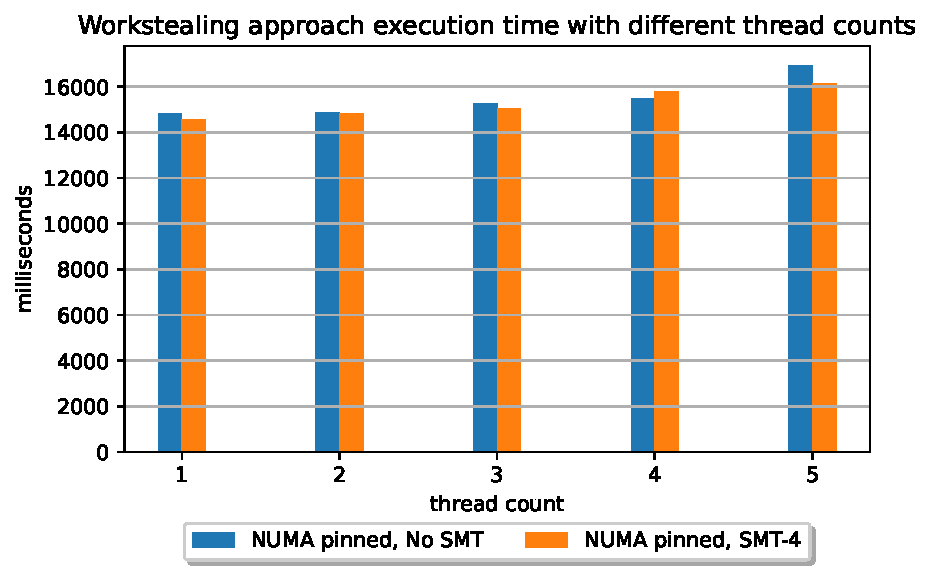
\includegraphics[width=\textwidth]{figures/ac922_threadcount.pdf}
  \centering
  \label{fig:threadcount_ac922}
\end{figure}

For a better understanding of the bottleneck in those benchmarks, a few benchmarks with different AC922 CPU influencing settings are done in Figure \ref{fig:threadcount_ac922}. A tendency to better performance can be seen for fewer threads. The difference between SMT-4 and no SMT is small and insignificant. With an execution time of 14560.6 ms, the NUMA pinned SMT-4 version is the fastest and does not show the bottleneck of the first AC922 benchmarks. It is around ten times faster than the AC922 NUMA-pinned max threads workstealing execution and around \textbf{13,8\% faster} than the GPU-only execution on the AC922 system. Therefore a performance improvement using the heterogeneous computing approach can be seen in comparison to the GPU-only execution. The comparison in Figure \ref{fig:threadcount_ac922} shows a slowdown with additional threads, which indicates a parallelism problem in the CPU code or bad Power9 optimization. A detailed investigation of the CPU parallel performance is left for future work.

\paragraph{Level-wise TCGA-1000 Benchmark}
\begin{figure}[H]
  \caption{Comparing the workstealing approach pinned to a NUMA node and 1 CPU execution thread, level-wise (AC922)}
  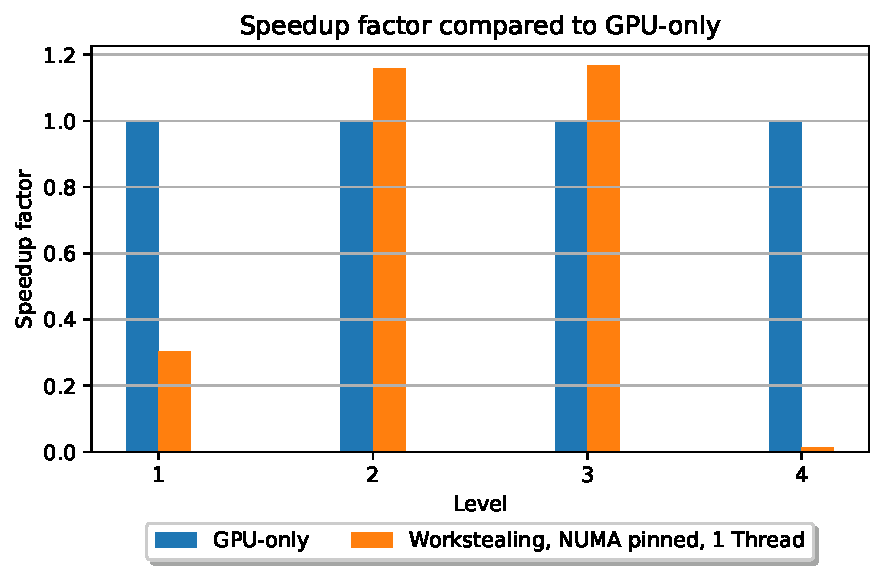
\includegraphics[width=\textwidth]{figures/ac922_levelwise.pdf}
  \centering
  \label{fig:levelwise_ac922}
\end{figure}

By measuring the level-wise impact in \ref{fig:levelwise_ac922} the same behavior as in the Delos level-wise benchmarks can be seen. Levels 2 and 3 profit from the heterogeneous computation, but levels 1 and 4 are slowed down. A slight performance improvement would be achievable by switching the approaches in an intelligent way per level. Nevertheless, the same relative distribution of time spent can be observed here, and levels 1 and 4 only make up a small percentage of the total execution time.

\subsection{Delos versus AC922}
In Chapter \ref{chap:setup} while explaining the setup, the differences between PCIe 3.0, incorporated in the Delos system between the CPU and GPU, and NVLink 2.0, incorporated in the AC922 system between the CPU and the GPU, are investigated. While NVLink has better throughput and latency than PCIe 3.0, comparing both systems might lead to insights into the impact of the interconnect.

Further, the Delos Intel Xeon Gold 6148 performs presumably better than the Power9 CPU in the AC922 system \cite{POWER9BenchmarksVs}, which could also invalidate the gains through the better interconnect of the AC922 system.

\begin{table}[H]
  \centering
  \begin{tabular}{||c | c | c||} 
   \hline
    & Execution time Delos (ms) & Execution time AC922 (ms) \\ [0.5ex] 
   \hline\hline
   GPU-only & 16290.8 & 16577.2 \\
   Workstealing & 13983.2 & 14560.6 \\ [1ex] 
   \hline
  \end{tabular}
  \caption{Comparing the best workstealing approach execution times of both the Delos and the AC922 system}
  \label{table:ac922_vs_delos}
\end{table}

The execution times are seen in \ref{table:ac922_vs_delos} show that the Delos system workstealing execution with a speedup of 16,5\% versus the GPU-only variant is a bit faster than the AC922 system workstealing execution with a speedup of 13,8\% versus the GPU-only variant.

The interconnect factor does not show the expected performance improvements results. The implementation of both approaches is aligned to the strict separation of reads and writes between tasks on the same data. The observation that the interconnect does not strongly influence the performance of the execution implies that the separation of reads and write on the same data is successful. The better performance of the Delos CPU can compensate for any gains of the AC922 system through the interconnect.

% - Explain dataset used for testing (TCGA)
%   - Variable size
%   - how sampled
%   - paper (perscheid etc)
% - Show delos as a testing machine
%   - Intel Xeon 
%   - Nvidia  V100
%   - specs
%   - numa nodes
% - Show AC922
%   - Explain why power9 + V100 special
%   - ATS: Malloc is enough
%   - Faster interconnect NVLINK
%     - Comparison between interconnects
%   - Other pros : atomics etc
%   - Explain why this should affect my performance
%   - Compare Power9 to Intel Xeon
% - Show iteration measurements per level
%   - show how many tests and iterations have to be done

% - Measurements of GPU only Code

% - Measurements of Pre-balanced
%   - With, without migrating edges
%   - Different thresholds
%   - Different Dataset sizes
%   - Different omp scheduling methods
%   - Pinning on NUMA nodes
%   - Delos vs AC922
% - Measurements of Workstealing
%   - With, without migrating edges
%   - Different Dataset sizes
%   - Pinning on NUMA nodes
%   - Delos vs AC922

% - Measurements with different Datasets
%   - Iterations
%   - Workstealing Numa 0
%   - Prebalanced
%   - GPU only
